\section{Motivation}
Semiconductor detectors play an important role in the detection of particles at experiments like ATLAS at the Large Hadron Collider (LHC) at CERN. 
In this experiment, the characteristics of a silicon strip sensor and its readout electronics are examined with a Educational Alibava
System (EASy).
Particle interactions stimulated by a laser and a strontium-90 source are measured and the data is processed and analysed.

\section{Theory}
\label{sec:Theory}
Silicon strip sensors are semiconductor detectors which are used to measure particle tracks. For example, the \textit{Inner Detector} (ID) at ATLAS is composited of
the \textit{Pixel Detector} in the innermost layers and the \textit{Silicon Strip Detector} (SCT).
When compared to higher resolution pixel sensors, silicon strip sensors offer a good trade off between spatial resolution and cost effectiveness.  
The working principle of such detectors is discussed in the following chapter.

\subsection{Semiconductors}
\label{subsec:Semiconductors}
The conduction properties of a material are defined by their electron bands. The gap between the highest filled band (valence band) and the lowest unfilled band (conduction band)
is called bandgap. Depending on the bandgap, materials are categorised as metals, semiconductors or insulators as shown in \autoref{fig:bandgap}.
\begin{figure}
    \centering 
    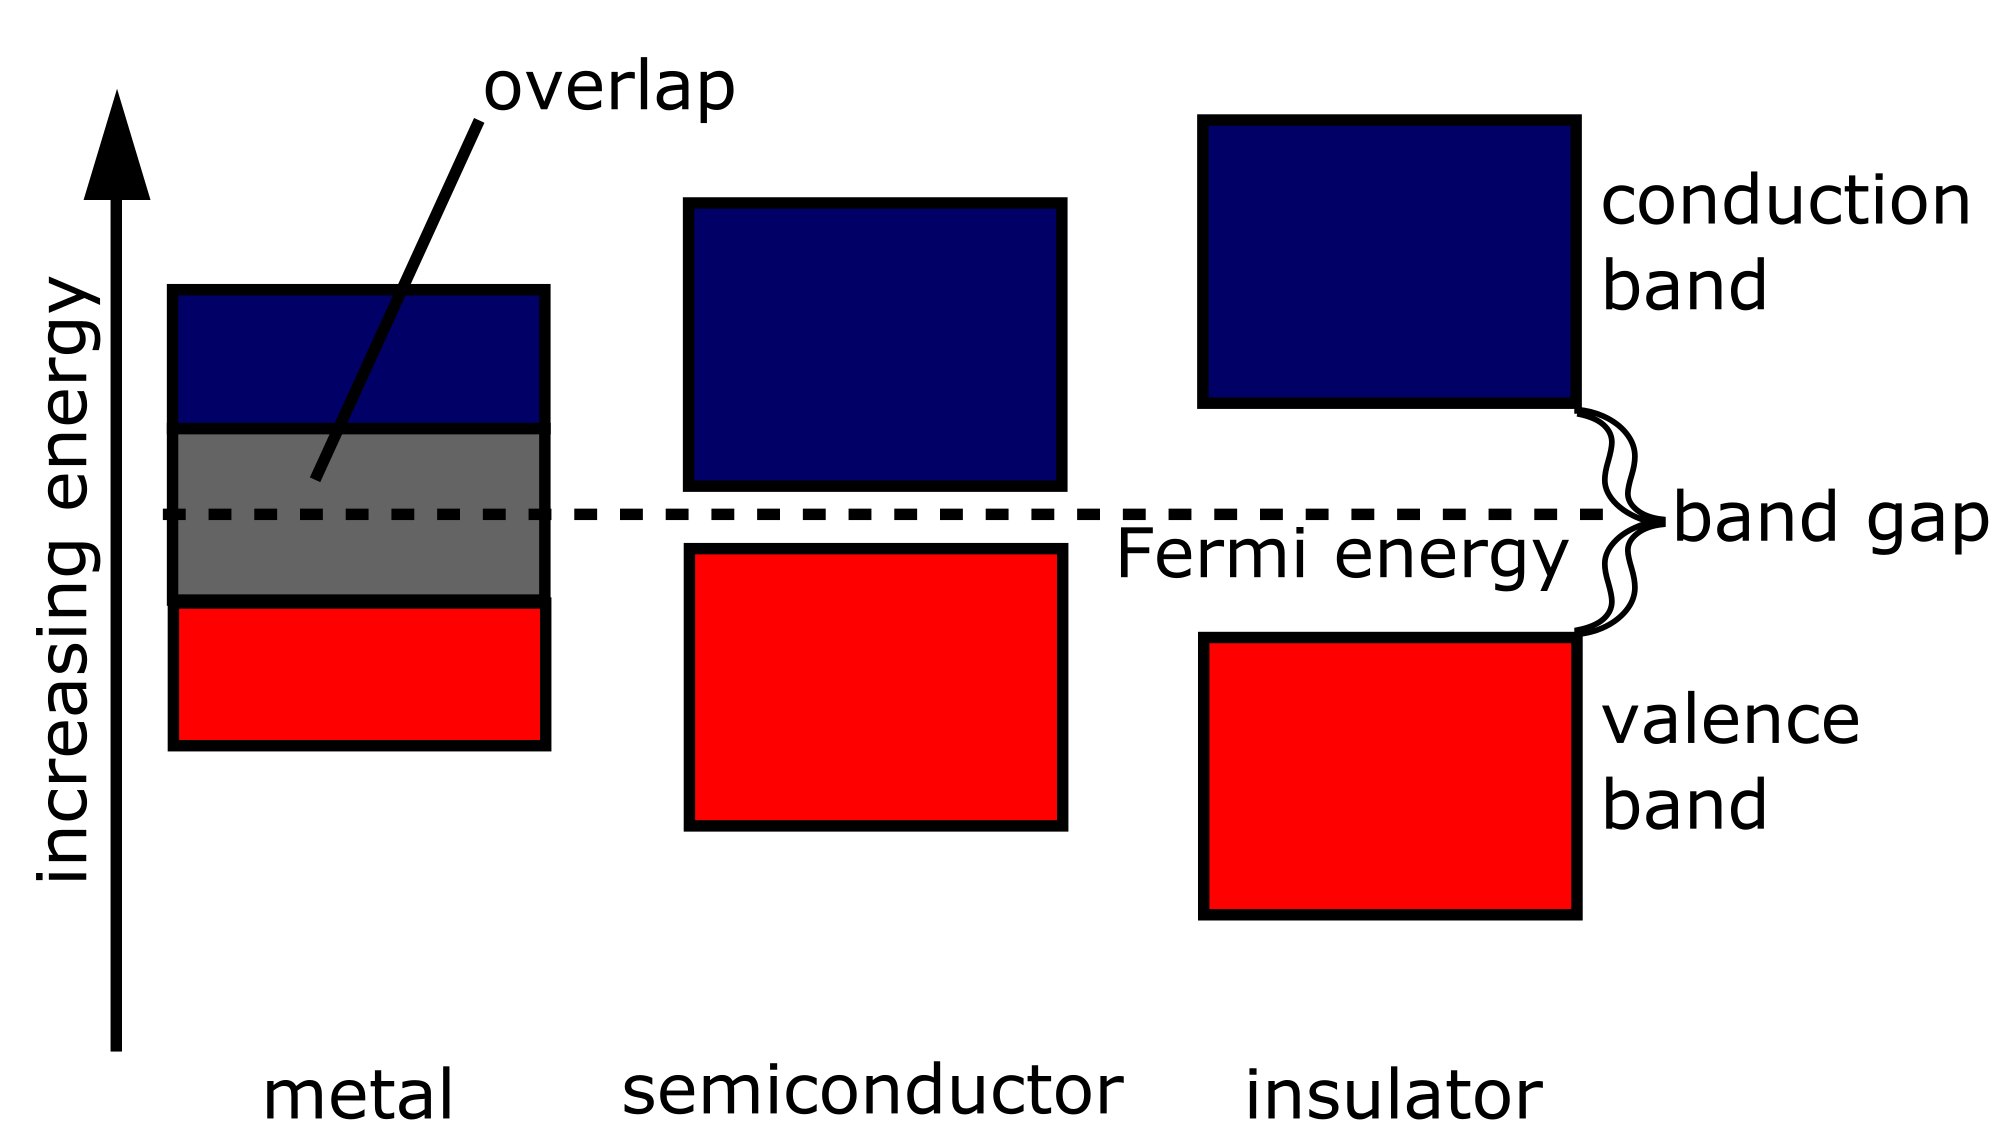
\includegraphics[width = .6\textwidth]{content/pics/Band_gap.png}
    \caption{Electron bands for different types of materials \cite{Bandgap}.}
    \label{fig:bandgap}
\end{figure}
Metals are characterised by overlapping conduction and valence bands and have no bandgap, therefore they are conductive. 
For insulators, the band gap is around $\qty{4}{\eV}$ or higher, which is why they are not conductive because the energy from thermal excitation 
is much smaller ($\approx\qty{30}{\milli\eV}$). Semiconductors typically have a bandgap of 1 to $\qty{5}{\eV}$ and are also not conductive at 
$T = \qty{0}{\kelvin}$. However, at roomtemperature electrons can be excited to the conduction band. The \enquote{hole} that they leave behind can be viewed as a quasiparticle that 
carries a positive charge and has an effective mass. Silicon, which is used for the detector in this experiment, has a bandgap of $\qty{1.107}{\eV}$ and an intrinsic charge 
carrier density of $\qty{1.5e10}{\centi\metre^{-3}}$. Silicon belongs to the \textit{element semiconductors}, other types are \textit{compound semiconductor} 
like gallium arsenide or \textit{organic semiconductors} which consist of carbon compounds.

\subsection{Doping of semiconductors}

The intrinsic charge carrier density for pure (= intrinsic) semiconductors is often too small to effectively use them. Therefore, atoms with a different amount of 
valence electrons are introduced
into the crystal structure of a semiconductor to increase its conductivity. This process is called doping. Silicon has 4 valence electrons and forms a diamond lattice structure. 
Silicon doped with pantavalent atoms, such as arsenic, is called a \textit{n-type} semiconductor. The fifth valence electron is not needed in the crystal bond and acts as a free 
charge carrier on a new level in the band diagram right below the conduction band which is called \textit{donator level}. This effectively reduces the band gap. 
Electrons in the donator level can easily be excited to the conduction band which inreases conductivity. \\
Alternatively, trivalent atoms, like boron, can be used. The semiconductor is then called \textit{p-type}. The missing electron in the bond can be seen as a hole, that can
move freely in the coulomb potential of the crystal lattice. A new level, called \textit{acceptor level}, arises in the band diagram right above the valence band.
Electrons from the valence band can be excited to the acceptor level.
The two types of doping are visualised in \autoref{fig:doping}.
\begin{figure}
    \centering 
    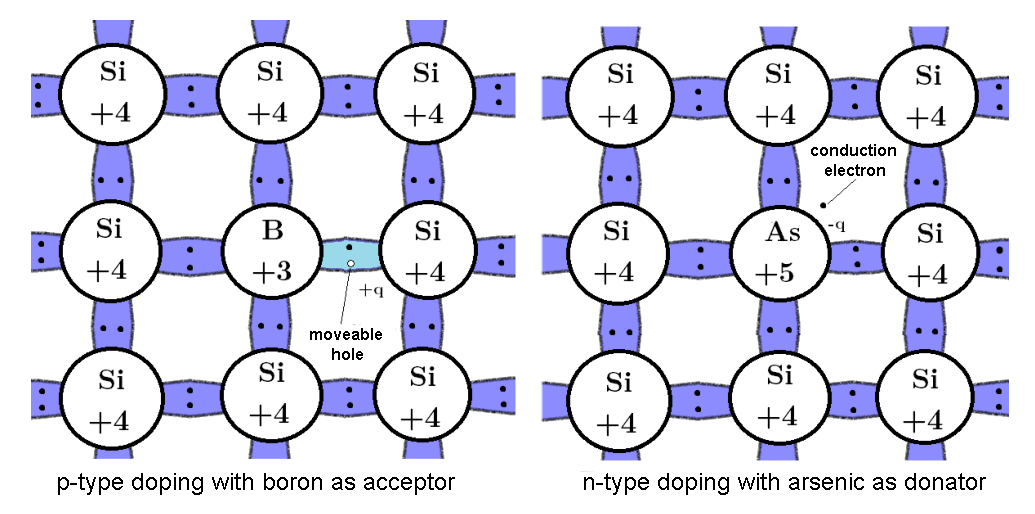
\includegraphics[width = .75\textwidth]{content/pics/doping.png}
    \caption{Schematic representation of an n- and p-type doped silicon semiconductor (Adapted from \cite{SiliconStrip}).}
    \label{fig:doping}
\end{figure}

\subsection{The pn-junction}
By connecting a n-type to a p-type semiconductor, a diode can be created. At the transition between the n- and p-type semiconductors (the \textit{pn-junction}) electrons from the 
n-side and holes from the p-side diffuse towards the respective other side and recombine. Because of the recombination, no free charge carriers remain at the junction.
The stationary doping atoms are now missing an electron or hole and cause a positive charge at the n-side and a negative charge at the p-side, resulting in an electric field.
Through the electric field, the remaining charge carriers drift in the opposite direction. When equilibrium is reached between drift and diffusion, a zone around the pn-junction 
with no charge carriers is created - the \textit{depletion zone}. The difference in the potential of the two sides is called diffusion voltage $U_D$.
By applying an external electric field (bias voltage), this effect is either weakened (+ on p-side, - on n-side) and a light emitting diode is created, or the effect is amplified 
(+ on n-side, - on p-side) which increases the thickness of the depletion zone. This is the case for the detector operation of the diode. Electron-hole pairs created in the
depletion zone (e.g. by a traversing particle) are drawn to the p- and n-side which generates a measurable current.
The thickness of the depletion zone depends on the applied voltage and can be calculated as 
\begin{equation}
    d(U) = \sqrt{\frac{2\varepsilon (U_D + U)}{qN_\text{eff}}},
    \label{eq:depletion_zone}
\end{equation}
where $\varepsilon$ is the dielectric constant of the material and $N_\text{eff}$ is the effective charge carrier density of the crystal.
It is given by 
\begin{equation}
    N_\text{eff} = \frac{N_D N_A}{N_D + N_A},
    \label{eq:N_eff}
\end{equation}
where $N_D$ and $N_A$ are the doping concentrations of the donors and acceptors, respectively.
For the detector operation, the whole crystal should be depleted, requiring a minimum depletion voltage of $U_\text{dep}$. Using \autoref{eq:depletion_zone} and neglecting 
the diffusion voltage $U_D$, $U_\text{dep}$ can be calculated via
\begin{equation}
    U_\text{dep} \approx \frac{q}{2\varepsilon} N_\text{eff} D^2.
    \label{eq:U_dep}
\end{equation}
Here, $D$ is the thickness of the sensor.
With $U_\text{dep}$ given, the thickness $d_c$ of the depletion zone can be approximated via 
\begin{equation}
    d_c(U) = 
    \begin{cases}
        D \sqrt{U/U_\text{dep}} & , U<U_\text{dep} \\
        D & , U \geq U_\text{dep}.
    \end{cases}
\end{equation}

Ideally, only energy deposition of ionising particles causes a current. In reality however, electron-hole pairs are also created by thermal excitation and are drawn to the poles,
causing a \textit{leakage current}. The leakage current increases with the bias voltage. In \autoref{fig:leakage_current}, a measured leakage current for the system used here,
is plotted against the bias voltage. 
\begin{figure}
    \centering 
    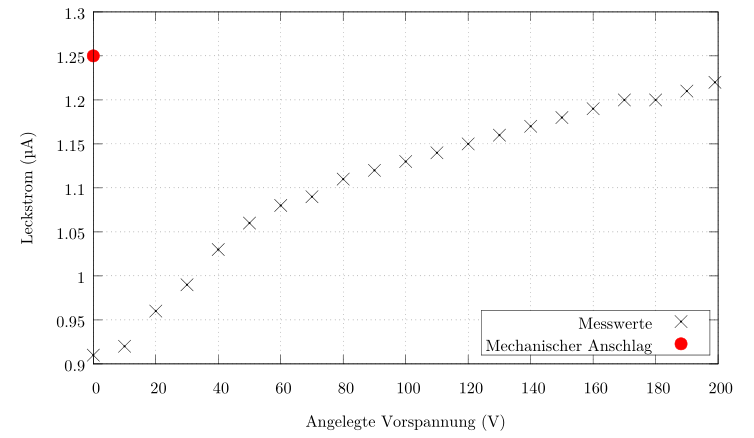
\includegraphics[width = .75\textwidth]{content/pics/leakage_current.png}
    \caption{Measurement of the leakage current against the bias voltage for the Educational Alibava system used in this experiment \cite{SiliconStrip}. 
    The depletion voltage can be read from the plot as $\qty{60}{\volt}$.}
    \label{fig:leakage_current}
\end{figure}
As can be seen from the plot, the leakage current strongly increases, till the depletion voltage $U_\text{dep}$ is reached and then continues to increas linearly.
From this measurement, the depletion voltage can be obtained.

\subsection{Interaction of ionising radiation with matter}
In this experiment, the EASy detector system is employed to measure ionising particles from a strontium-90 source. 
Therefore it is important to understand the energy deposition of ionising particles in matter.

\subsubsection{The beta decay}
In general, the beta decay proceeds over 
\begin{equation*}
    n \to p + e^- + \bar{\nu_e}.
\end{equation*}
The free binding energy is randomly distributed to the decay products (i.e. the electron and neutrino), resulting in an energy spectrum of the electron as shown in 
\autoref{fig:beta_spectrum}.
\begin{figure}
    \centering 
    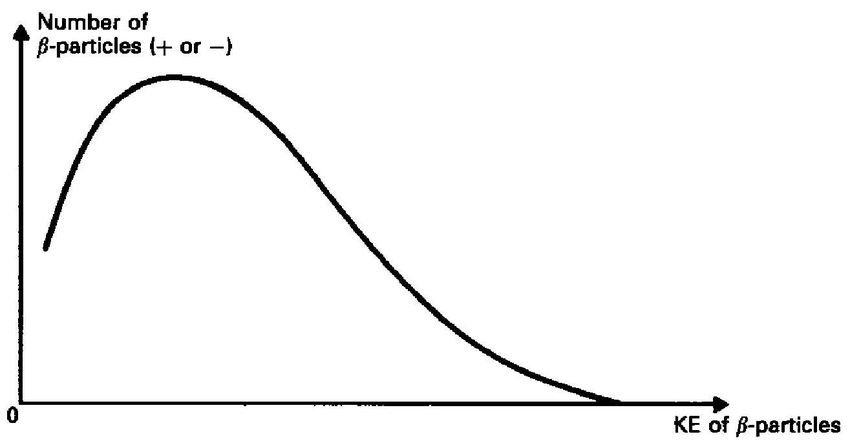
\includegraphics[width = .75\textwidth]{content/pics/beta_spectrum.png}
    \caption{Electron energy spectrum of a $\beta^-$ decay \cite{beta_spectrum}.}
    \label{fig:beta_spectrum}
\end{figure}
As can be seen in the plot, a material dependent maximum energy can be reached.
The decay chain of strontium-90 is 
\begin{equation*}
    \ce{^{90}{Sr}} \xrightarrow{\beta^-} \ce{^{90}{Y}}  \xrightarrow{\beta^-} \ce{^{90}{Zr}}.
\end{equation*}
The strontium has a half-life of $\qty{28.78}{\year}$ while yttrium has a half-life of $\qty{59}{\day}$ and the zirconium is stable.
Both \ce{^{90}{Sr}} and \ce{^{90}{Y}} decay via the $\beta^-$ decay. The maximum kinetic energy of the electron is $\qty{0.546}{\mega\eV}$ and $\qty{2.28}{\mega\eV}$ for 
strontium and yttrium, respectively \cite{Leo1987}.
For a simple 1-step decay chain, the activity (decays per time) is given by 
\begin{equation*}
    A(t) = - \frac{\symup{d}N}{\symup{d}t} = \lambda N_0 \mathrm{e}^{-\lambda t},
\end{equation*}
with the initial number of atoms $N_0$ and the decay constant $\lambda$ of the atom. The unit is $\unit{\becquerel} = \unit{\second^{-1}}$.
For a decay chain, this is more complicated, but in the limit $T_{1/2, \ce{^{90}{Sr}}} \gg T_{1/2, \ce{^{90}{Y}}}$ the total activity is effectively the \ce{^{90}{Sr}} 
activity doubled.

\subsubsection{Interactions of electrons in matter}
When traversing a material, the electrons interact with the nucleus and electrons of the atomic shell and deposit energy. Since the kinetic energy of the electrons in this experiment
is not large enough, bremsstrahlung, inelastic collisions with the nuclei and Cherenkov radiation are not considered. The relevant effect here, is the ionisation of the atoms by 
collisions of the incoming electrons with shell electrons. The average energy loss per distance of the electron is given by the modified Bethe-Bloch equation \cite{Leo1987}
\begin{equation}
    -\frac{\symup{d}E}{\symup{d}x} = 2 \mathrm{\pi} N_\text{A} m_e c \rho \frac{Z}{A} \frac{1}{\beta^2}
    \left[ \symup{ln}\left(\frac{\tau^2(\tau +2)}{2(I/m_ec^2)^2}\right) + F(\tau) -\delta -2 \frac{C}{Z}\right].
    \label{eq:bethe_bloch}
\end{equation}
Here, $Z$ and $A$ are the proton- and mass number of the material, $\rho$ the materials density, $m_e$ is the electron mass, $c$ the speed of light, 
$\beta$ the relativistic beta factor, $N_\text{A}$ the Avogadro constant and $\delta$ and $C$ the density and envelope corrections. $I$ is the average excitation potential and 
$\tau = 1 - \gamma$ corresponds to the kinetic energy of the electron. $F(\tau)$ is determined as
\begin{equation*}
    F(\tau) = 1-\beta^2 + \frac{\frac{\tau^2}{8}- (2r_e + 1)\symup{ln}(2)}{(\tau+1)^2}
\end{equation*}
with $r_e$ the classic electron radius. For \ce{^{90}{Sr}} it follows, that an electron of maximum energy deposits an energy of $\qty{3.88}{\mega\eV\per\cm}$ in pure 
silicon \cite{SiliconStrip}. \\
In this experiment, the spectrum of energy deposition of the electrons in the silicon can best be described by a convolution of a Gaussian- and a Landau- distribution as shown
in \autoref{fig:energy_deposition}.
\begin{figure}
    \centering 
    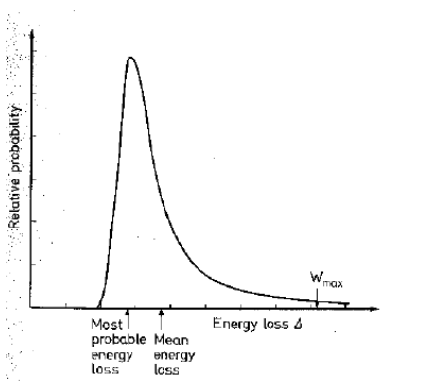
\includegraphics[width = .5\textwidth]{content/pics/energy_deposition.png}
    \caption{Energy depostion of electrons in a $\qty{300}{\micro\meter}$ silicon sensor \cite{SiliconStrip}.}
    \label{fig:energy_deposition}
\end{figure}

\subsection{Pedestals and Noise}
In this experiment, the charge deposition is given in counts of the analogue-to-digital converter (ADC counts) and therefore has to be converted to $\unit{\kilo\eV}$ 
on the basis of a callibration measurement. The callibration generates a specified amount of electron-hole pairs which are then converted into ADC counts.
To create one electron-hole pair in silicon, an energy of $\qty{3.6}{\eV}$ \cite{SiliconStrip} is required.

When measuring, the ADC counts always include noise. In order to get the signal count, all unwanted effects have to be subtracted.
In total, the measured ADC counts for a signal $k$ at strip $i$ is given by 
\begin{equation}
    \text{ADC}(i, k) = \text{P}(i, k) + \text{D}(i,k) + \text{Signal}(i, k) + \text{Noise}(i, k).
    \label{eq:ADC}
\end{equation}    
The \textit{pedestal} $\text{P}(i, k)$ is the mean value of ADC counts for a strip without external signal and can be calculated via 
\begin{equation}
    \text{P}(i) = \frac{1}{N} \sum^N_{k = 1} \text{ADC}(i,k)
    \label{eq:pedestals}
\end{equation}
from $N$ measurements without signal. $\text{D}(k)$ is called the \textit{Common Mode Shift} or \textit{Common Noise} and describes a global disturbance affecting all 
strips during an event and can be determined as 
\begin{equation}
    \text{D}(k) = \frac{1}{128} \sum^{128}_{i = 1} (\text{ADC}(i,k) -\text{P}(i)).
    \label{eq:common_noise}
\end{equation}
The common noise is gaussian distributed around 0.
Finally, the noise of each strip can be calculated using the root-mean-square of the ADC counts after subtracted pedestals and common noise:
\begin{equation}
    \text{Noise}(i) = \sqrt{\frac{1}{N-1} \sum^{N}_{k = 1} (\text{ADC}(i,k) -\text{P}(i) - \text{D}(k))^2}.
    \label{eq:noise}
\end{equation}
When measuring a true signal, this calculation has to be performed a second time, where signals several standard deviations above the noise level are then sorted out.

